\chapter{Research Methodology and System Design}

Every chapter should start with 1-2 sentences on the outline of the chapter. [This chapter outlines the research methodology, stakeholder analysis, functional and non-functional requirements, system architecture, hardware BOM, network design, and relational database models.]

\section{Research Methodology}
[Detail the research lifecycle, phases, iterative development workflow, and empirical validation plan.]

\section{Stakeholder and Requirements Analysis}
\subsection{Stakeholder Analysis}
\begin{table}[H]
\centering
\caption{Stakeholder Analysis and System Needs Mapping}
\label{tab:template_stakeholders_ch3}
\small
\begin{tabularx}{\textwidth}{>{\raggedright\arraybackslash}p{3.0cm} >{\raggedright\arraybackslash}p{4.0cm} >{\raggedright\arraybackslash}X}
\toprule
\textbf{Stakeholder Group} & \textbf{Core Role / Context} & \textbf{System Needs \& Expectations} \\
\midrule
\textbf{[Stakeholder 1]} & [Primary role] & [Core requirements expected from system]. \\
\textbf{[Stakeholder 2]} & [Secondary role] & [Core requirements expected from system]. \\
\textbf{[End Users]} & [Direct users] & [User experience and operational needs]. \\
\bottomrule
\end{tabularx}
\end{table}

\subsection{Functional Requirements Specification}
\begin{table}[H]
\centering
\caption{Functional Requirements Specification (FRS) Matrix}
\label{tab:template_frs_ch3}
\small
\begin{tabularx}{\textwidth}{>{\centering\arraybackslash}p{1.6cm} >{\raggedright\arraybackslash}p{4.0cm} >{\raggedright\arraybackslash}X >{\centering\arraybackslash}p{1.6cm}}
\toprule
\textbf{Req ID} & \textbf{Requirement Title} & \textbf{Functional Description} & \textbf{Priority} \\
\midrule
FR-01 & [Data Ingestion / Capture] & [Detailed description of functional behavior]. & High \\
FR-02 & [Core Processing / Algorithm] & [Detailed description of functional behavior]. & High \\
FR-03 & [Storage / Database] & [Detailed description of functional behavior]. & High \\
FR-04 & [User Interface / Alerts] & [Detailed description of functional behavior]. & Medium \\
\bottomrule
\end{tabularx}
\end{table}

\section{System Architecture and Component Design}
\begin{figure}[H]
\centering
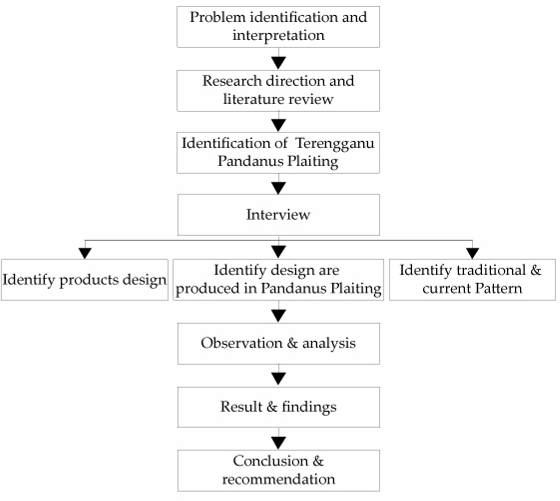
\includegraphics[width=0.85\textwidth]{./media/image2.png}
\caption{High-Level System Architecture Diagram}
\label{fig:template_sys_arch_ch3}
\end{figure}

\section{Hardware Architecture and Bill of Materials (BOM)}
\begin{table}[H]
\centering
\caption{Hardware Bill of Materials (BOM) and Cost Breakdown}
\label{tab:template_bom_ch3}
\small
\begin{tabularx}{\textwidth}{>{\raggedright\arraybackslash}p{2.8cm} >{\raggedright\arraybackslash}X >{\raggedright\arraybackslash}X >{\raggedleft\arraybackslash}p{2.0cm}}
\toprule
\textbf{Component} & \textbf{Model / Specifications} & \textbf{Operational Role} & \textbf{Est. Cost (BDT)} \\
\midrule
{[Microcontroller]} & {[e.g., ESP32 / Arduino / Raspberry Pi]} & {[Sensor reading and networking]} & [Cost] \\
{[Primary Sensor / Camera]} & {[Model / Part Number]} & {[Data collection / vision capture]} & [Cost] \\
{[Power / Enclosure]} & {[Regulator / Battery / Case]} & {[Power regulation and protection]} & [Cost] \\
\midrule
\multicolumn{3}{l}{\textbf{Total Hardware Prototyping Cost}} & \textbf{[Total BDT]} \\
\bottomrule
\end{tabularx}
\end{table}

\section{Data Flow Modeling (DFD)}
\subsection{Context Diagram (DFD Level 0)}
[Explain external entities, inputs, and outputs.]

\subsection{Decomposed Data Flow Diagram (DFD Level 1)}
[Detail sub-processes, data stores, and internal data flows.]

\section{Database Design and Relational Schema (ERD)}
\begin{figure}[H]
\centering
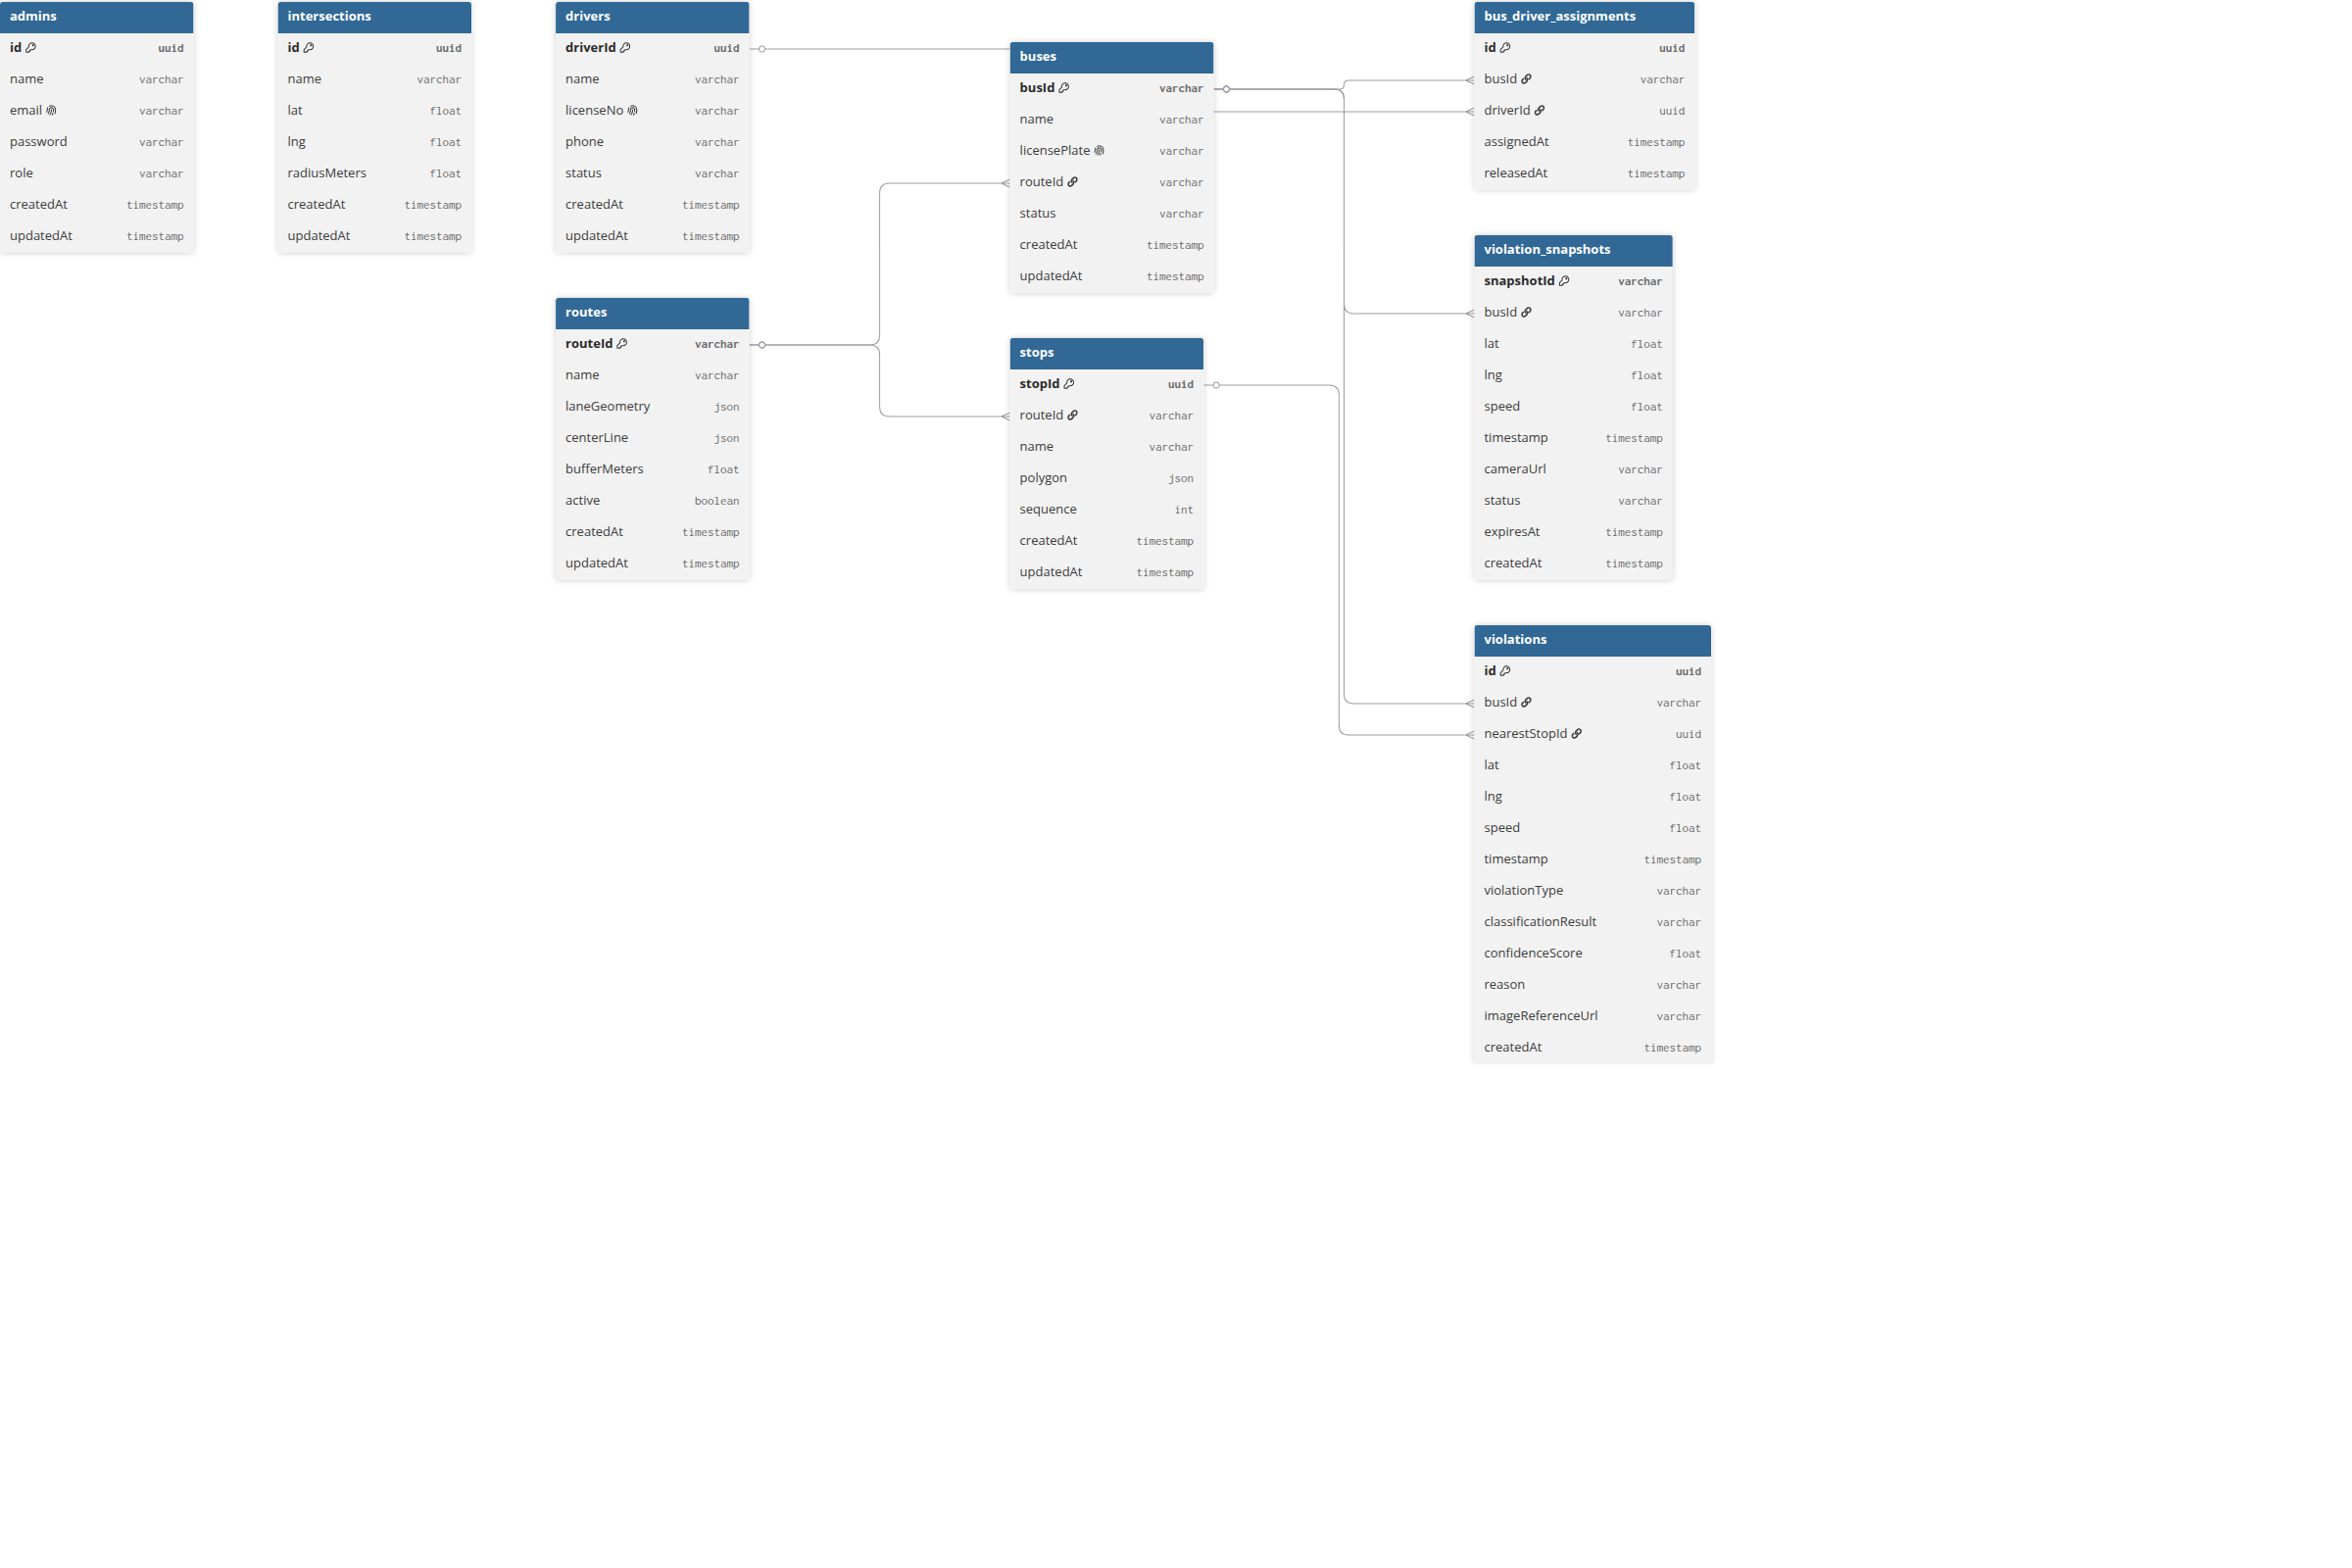
\includegraphics[width=0.90\textwidth]{./media/final_ERD.png}
\caption{Relational Entity-Relationship Diagram (ERD)}
\label{fig:template_erd_ch3}
\end{figure}
